\title{\textbf{Page d'Accueil (Home)}}
\author{}
\date{}\documentclass[12pt,a4paper]{article}

% Paquetes básicos para idioma y formato
\usepackage[utf8]{inputenc}
\usepackage[T1]{fontenc}
\usepackage[french]{babel}
\usepackage{geometry}
\geometry{a4paper, margin=2.5cm}

% Paquetes para diseño y código
\usepackage{xcolor}
\usepackage{listings}
\usepackage{hyperref}
\usepackage{graphicx}
\usepackage{float}

% Configuración visual para los bloques de código JavaScript
\lstset{
    backgroundcolor=\color{gray!10},
    basicstyle=\ttfamily\small,
    keywordstyle=\color{blue}\bfseries,
    stringstyle=\color{red},
    commentstyle=\color{green!60!black},
    numbers=left,
    numberstyle=\tiny\color{gray},
    stepnumber=1,
    breaklines=true,
    frame=single,
    showstringspaces=false,
    language=Java % Usamos Java como base visual para JS
}

\title{\textbf{Rapport de Développement Web : Application Televerie}}
\author{
    \textbf{Projet réalisé par :} \\
    Facundo ARITO, Juan BAUDINO, Juan DE MIGUEL, Julian RAYES \\
    \textbf{Enseignant :} Sébastien KUBICKI \\
    \textbf{École Nationale d'Ingénieurs de Brest (ENIB)}
}
\date{}

\begin{document}

\maketitle
\thispagestyle{empty} % <-- Saca el número de la primera página (la del título)
\pagestyle{empty}     % <-- Saca el número de todas las páginas siguientes

\section*{Introduction Générale}
La société prestataire en charge des équipements de laverie des résidences CROUS de Brest nous a contactés pour résoudre un problème d'organisation majeur dans leurs locaux. Ce document s'inscrit dans la continuité de notre précédent rapport axé sur la conception centrée utilisateur (création des personas, idéation, wireframes, maquettes et prototype). 

L'objectif de ce nouveau rapport est de présenter la programmation technique du Frontend de l'application "Televerie". Nous y détaillerons la traduction de nos maquettes en code fonctionnel, en utilisant les langages web standards : HTML, CSS et JavaScript.

\section*{Comment lancer l'application}
Pour tester l'application "Televerie" sur votre ordinateur, plusieurs méthodes sont possibles. Veuillez suivre ces étapes selon la configuration de votre machine :

\subsection*{Méthode 1 : Ouverture directe}
La méthode la plus simple consiste à faire un double-clic sur le fichier \texttt{index.html}. Cela ouvrira l'application directement dans votre navigateur par défaut.

\subsection*{Méthode 2 : Configuration sur Firefox}
Si la première méthode ne fonctionne pas (parfois à cause des sécurités du navigateur bloquant les scripts locaux), nous recommandons d'utiliser Firefox :
\begin{itemize}
    \item Ouvrez Firefox et tapez \texttt{about:config} dans la barre d'adresse.
    \item Acceptez l'avertissement de sécurité.
    \item Cherchez le paramètre \texttt{privacy.file\_unique\_origin}.
    \item Changez sa valeur de \texttt{true} à \texttt{false}.
    \item Rechargez la page \texttt{index.html}.
\end{itemize}

% --- IMAGEN FIREFOX ---
\begin{figure}[H]
    \centering
    % Remplacez par le nom de votre image
    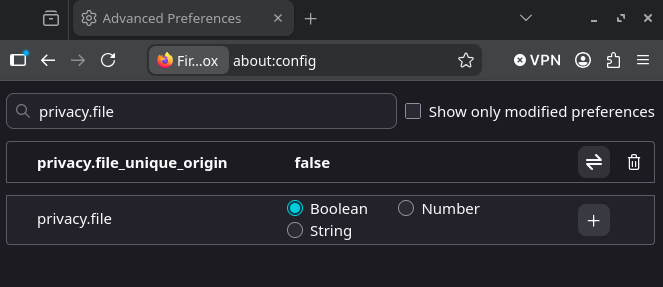
\includegraphics[width=0.8\textwidth]{firefox.png}
    \caption{Configuration du paramètre de confidentialité sur Firefox.}
\end{figure}

\subsection*{Méthode 3 : Lancer un serveur local (Python)}
Si les méthodes précédentes échouent, vous pouvez simuler un environnement de serveur web local via le terminal :
\begin{itemize}
    \item Ouvrez un terminal (ou l'invite de commandes).
    \item Naviguez jusqu'au dossier racine qui héberge le fichier \texttt{index.html}.
    \item Lancez la commande suivante : \texttt{python -m http.server}
    \item Ouvrez votre navigateur et accédez à l'adresse : \texttt{localhost:8000}
\end{itemize}

% --- IMAGEN TERMINAL ---
\begin{figure}[H]
    \centering
    % Remplacez par le nom de votre image
    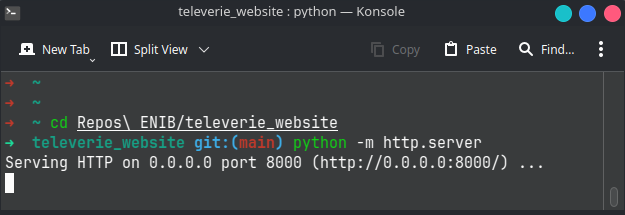
\includegraphics[width=0.6\textwidth]{konsole.png}
    \caption{Lancement du serveur local avec Python.}
\end{figure}

\begin{figure}[H]
    \centering
    % Remplacez par le nom de votre image
    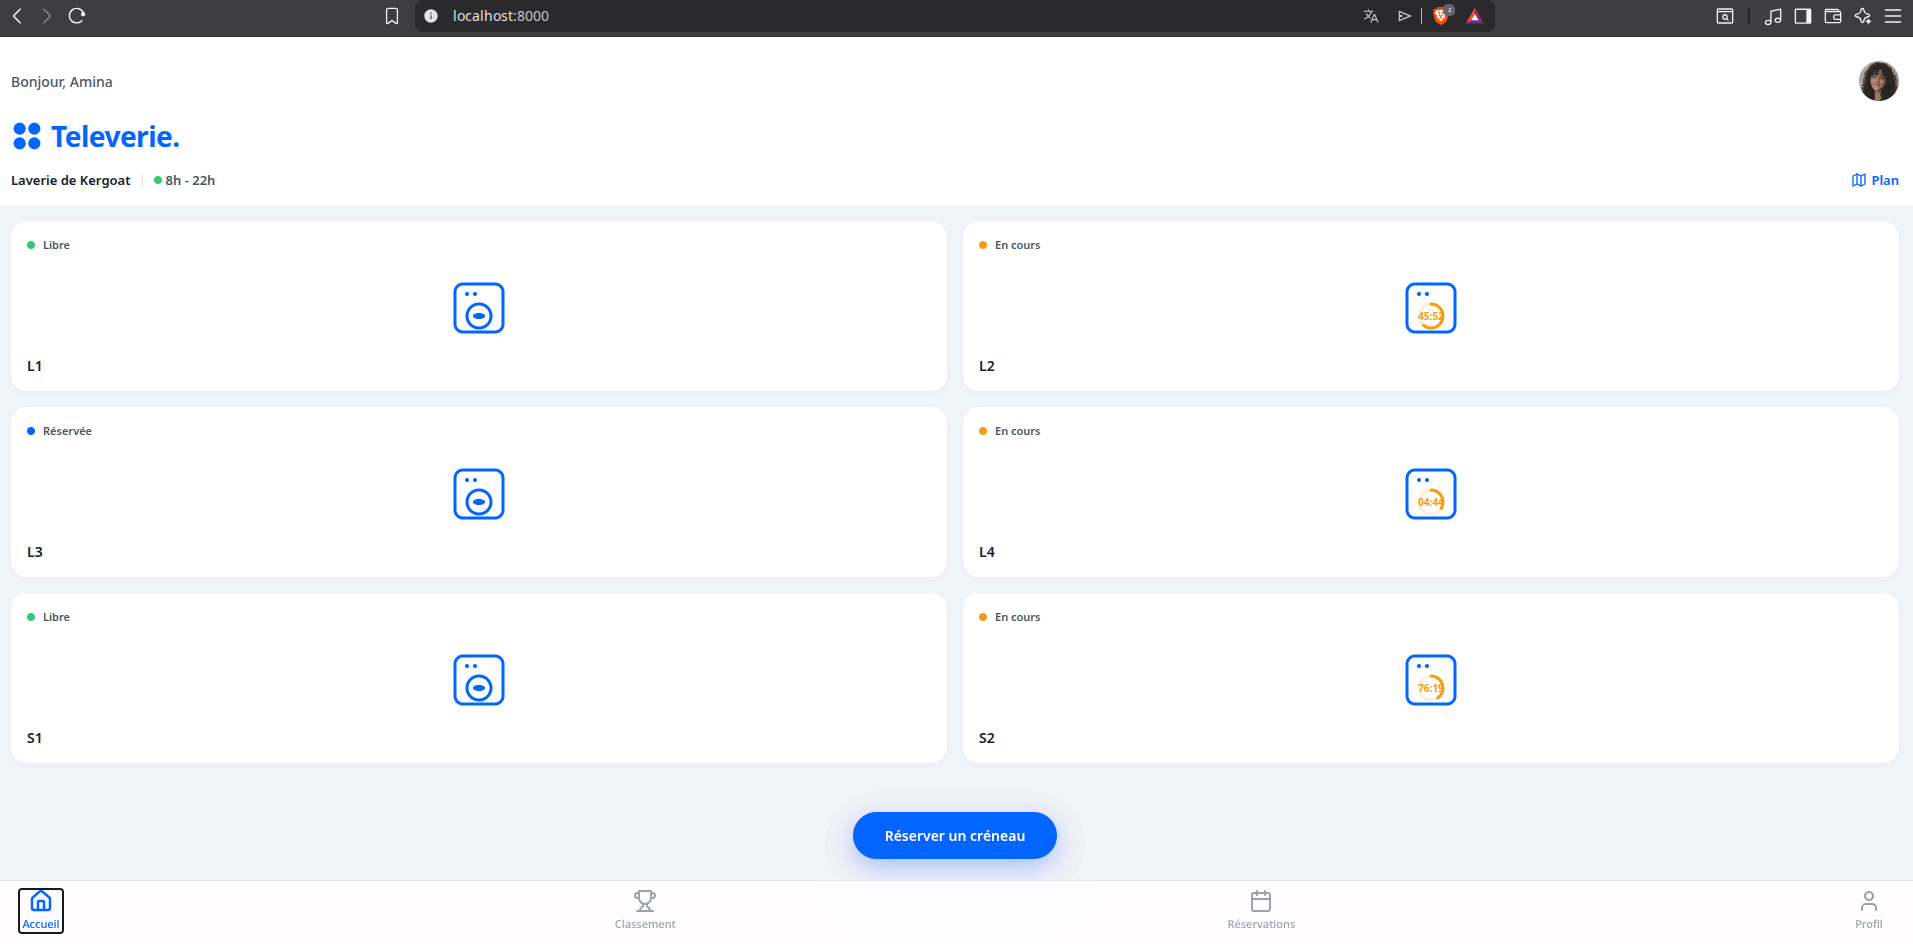
\includegraphics[width=0.8\textwidth]{localhost.png}
    \caption{Accès au serveur local.}
\end{figure}


\subsection*{Affichage en mode Mobile-First}
Une fois sur la page, l'application s'affichera à l'écran comme illustré avant, en mode PC.

Cependant, étant donné que "Televerie" est conçue avec une approche "Mobile-First", vous devez activer la vue mobile pour profiter d'une expérience optimale et fidèle au design :
\begin{itemize}
    \item Appuyez sur \texttt{Ctrl + Shift + I} (ou la touche \texttt{F12}) pour ouvrir les outils de développement du navigateur.
    \item Activez l'affichage "Appareil mobile" (souvent représenté par une icône de téléphone/tablette).
    \item Dans le menu déroulant en haut de l'écran, sélectionnez la vue \textbf{iPhone 14} ou \textbf{iPhone 14 Pro Max}.
\end{itemize}

% --- IMAGEN DEVTOOLS IPHONE ---
\begin{figure}[H]
    \centering
    % Remplacez par le nom de votre image
    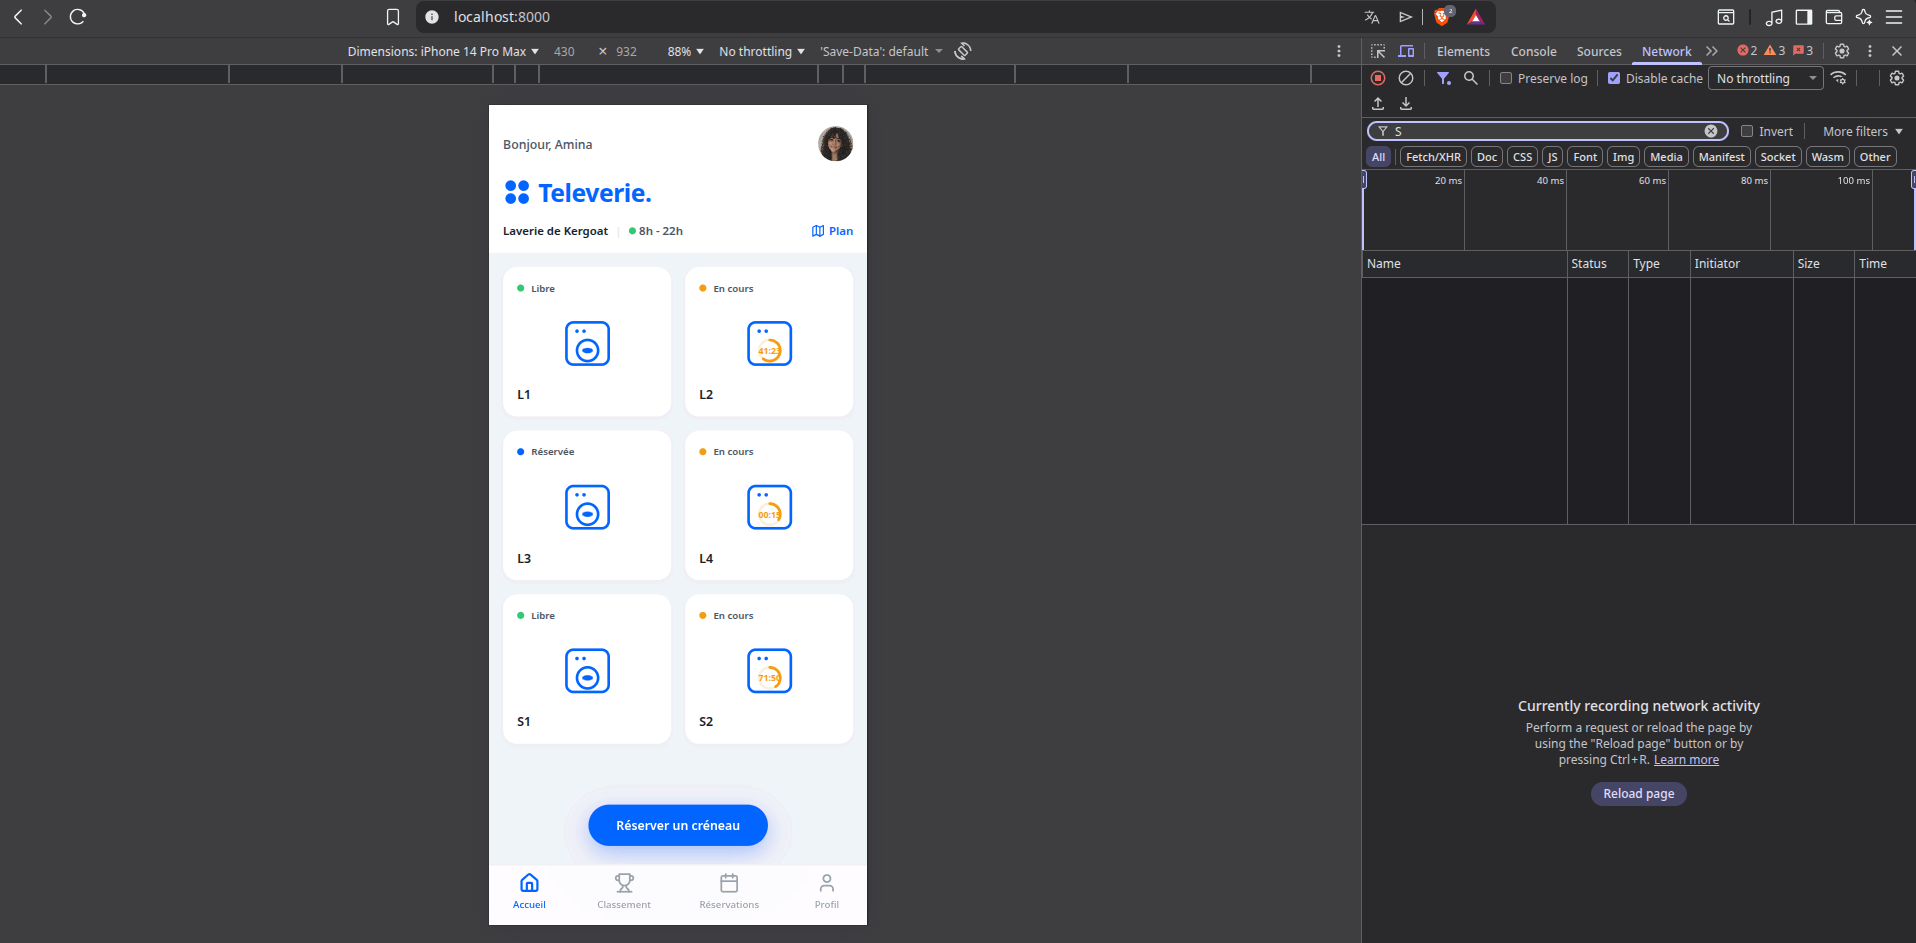
\includegraphics[width=0.8\textwidth]{mobile.png}
    \caption{Sélection de la vue iPhone 14 dans les outils de développement.}
\end{figure}

\newpage
\section*{Page d'Accueil}
\section*{Fonctionnalités de l'Accueil}
La page d'accueil est le tableau de bord principal de l'application. Son but est de donner à l'étudiant toutes les informations les plus importantes en un seul coup d'œil, pour qu'il ne perde pas de temps.

\begin{figure}[H]  % <--- LA "H" MAYÚSCULA HACE LA MAGIA
    \centering
    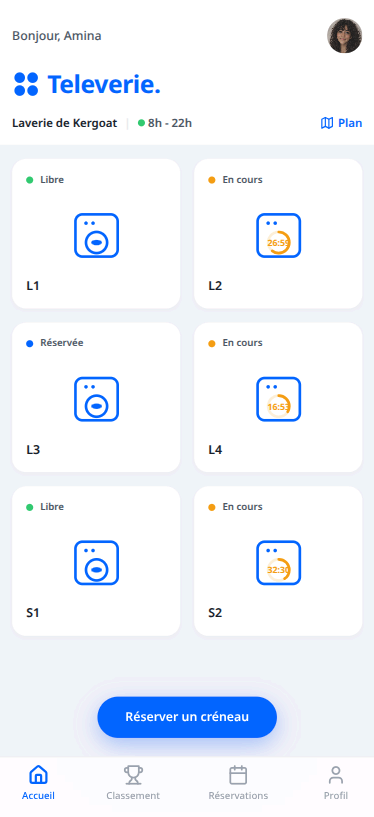
\includegraphics[width=0.4\textwidth]{pagedaccueil.png}
    \caption{Aperçu de la page d'accueil.}
    \label{fig:page-accueil}
\end{figure}

\subsection*{L'en-tête personnalisé}
En haut de l'écran, l'utilisateur est accueilli par son prénom (par exemple, "Bonjour, Amina") et sa photo de profil. Juste en dessous, l'application indique le nom de la laverie actuellement sélectionnée (comme "Laverie de Kergoat") et ses horaires d'ouverture (8h - 22h). Cet espace sert à rassurer l'utilisateur sur le lieu qu'il est en train de consulter. De plus, un bouton "Plan" est placé juste à côté pour permettre d'ouvrir rapidement une carte des résidences.

\subsection*{L'état des machines en direct}
Le centre de la page est composé d'une grille montrant 4 machines à laver et 2 sèche-linges. Pour rendre l'interface très visuelle et facile à comprendre, nous avons utilisé un code couleur simple pour indiquer le statut de chaque équipement :
\begin{itemize}
    \item \textbf{Vert (Libre) :} La machine est prête à être utilisée immédiatement.
    \item \textbf{Orange (En cours) :} La machine est occupée. Pour aider l'étudiant à calculer son temps, une animation circulaire avec un compte à rebours indique exactement les minutes restantes avant la fin du programme.
    \item \textbf{Bleu (Réservée) :} La machine est bloquée et attend l'arrivée de l'étudiant qui a réservé ce créneau.
\end{itemize}

\subsection*{L'action rapide (Bouton principal)}
Enfin, en bas de l'écran, un grand bouton bleu "Réserver un créneau" flotte au-dessus du contenu. Il s'agit de l'action principale de l'application. Un simple clic sur ce bouton connecte directement l'utilisateur au calendrier de réservation, ce qui rend l'expérience beaucoup plus fluide et rapide.

\section*{Navigation et Fenêtres Contextuelles (Pop-ups)}
Afin de rendre l'application plus fluide et d'éviter de recharger la page entière, nous avons intégré des "pop-ups" (ou fenêtres modales) directement sur la page d'accueil. Cette technique améliore considérablement l'expérience utilisateur (UX) car elle donne l'impression d'utiliser une véritable application mobile native. L'utilisateur reste toujours dans son contexte sans perdre le fil de sa navigation.

\subsection*{Pop-up de la Carte (Plan)}
En cliquant sur le bouton "Plan" situé en haut à droite de l'écran, une fenêtre superposée s'ouvre avec une carte interactive Google Maps intégrée. Cette carte montre avec précision 3 points (pins) rouges qui correspondent aux 3 résidences CROUS situées dans Brest Métropole. Cela est très utile pour les étudiants qui souhaitent vérifier la distance ou l'emplacement d'une autre laverie si la leur est complète. La fenêtre se ferme facilement en touchant la croix ou simplement en cliquant sur le fond sombre.

% --- ESPACE POUR L'IMAGE DE LA CARTE ---
\begin{figure}[H]  % <--- LA "H" MAYÚSCULA HACE LA MAGIA
    \centering
    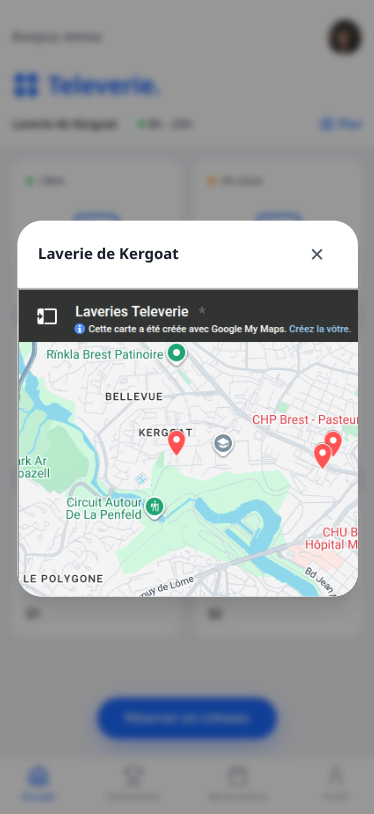
\includegraphics[width=0.4\textwidth]{popupmapa.png}
    \caption{Aperçu de la fenêtre modale affichant la carte interactive des résidences CROUS.}
    \label{fig:popup-carte}
\end{figure}

\subsection*{Pop-up du Profil Rapide}
Pour offrir un raccourci pratique, un clic sur la photo de profil ouvre un petit résumé des données de l'utilisateur. Par exemple, pour l'étudiante Amina Rahmani, le pop-up affiche son nom complet, son e-mail universitaire et son numéro de téléphone dans un design épuré avec des cadres blancs arrondis. En bas de ce pop-up, le bouton "Voir mon profil" permet de naviguer instantanément vers la section complète du compte.

\begin{figure}[H]
    \centering
    % Asegurate de que el archivo subido se llame exactamente popupmapa.png 
    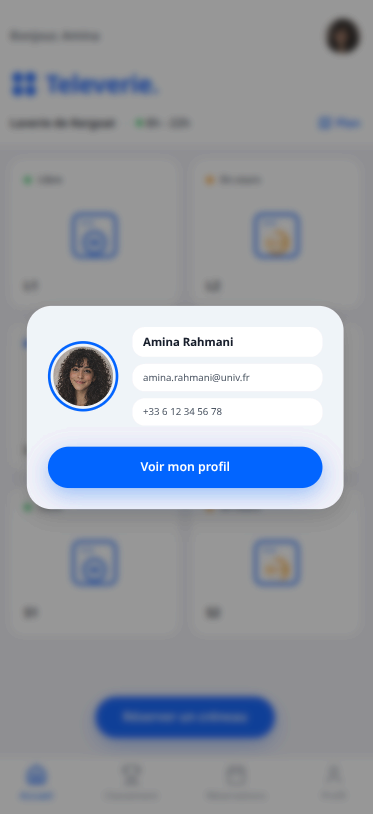
\includegraphics[width=0.4\textwidth]{popupprofil.png}
    \caption{Aperçu du pop-up de profil rapide avec les coordonnées basiques de l'utilisateur.}
    \label{fig:popup-profil}
\end{figure}

\subsection*{Pop-up de Réservation}
L'objectif principal de l'application est de permettre à l'utilisateur de réserver un créneau pour une machine spécifique à l'avance. Pour faciliter cette action fondamentale, le grand bouton bleu "Réserver un créneau", situé en bas de l'écran d'accueil, fait le lien direct. Lorsqu'on le touche, il simule une navigation vers l'onglet des réservations et indique au système d'ouvrir automatiquement la fenêtre modale du calendrier. L'étudiant peut ainsi choisir sa date et son heure immédiatement, ce qui lui fait gagner des clics.

% --- ESPACE POUR L'IMAGE DE RÉSERVATION ---
\begin{figure}[H]
    \centering
    % Asegurate de que el archivo subido se llame exactamente popupmapa.png 
    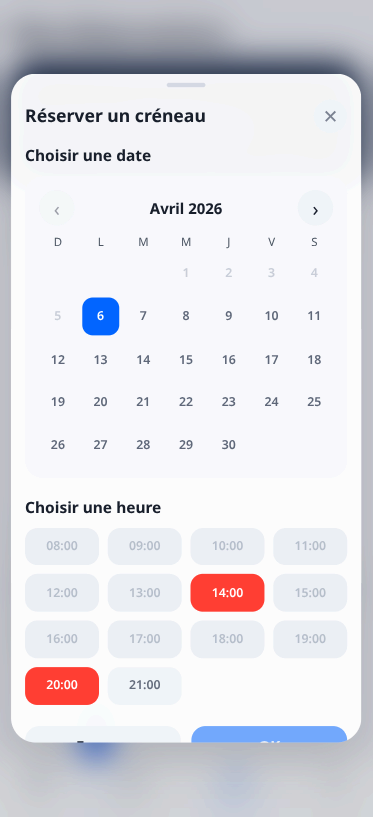
\includegraphics[width=0.4\textwidth]{popupreserv.png}
    \caption{Aperçu de la fenêtre modale de réservation avec le calendrier et les horaires.}
    \label{fig:popup-reservation}
\end{figure}

\section*{Détails Techniques : Le code \texttt{home.js}}
La logique interactive de cette page se trouve dans le fichier \texttt{home.js}.

\subsection*{Persistance des données (Le système de mémoire)}
L'un des défis techniques était de garder les chronomètres actifs même si l'utilisateur change d'onglet (par exemple, s'il va voir son profil puis revient à l'accueil). Pour résoudre cela, nous utilisons un objet \texttt{Map()} appelé \texttt{homeMachineEndTimes}. 
Lorsqu'une machine commence à tourner, le système enregistre son heure de fin dans cette "mémoire". Ainsi, quand la vue \texttt{initHomeView()} est rechargée, le code vérifie d'abord si la machine a déjà une heure de fin enregistrée avant de créer un nouveau chronomètre.

\subsection*{Un calcul du temps générique et automatique}
La fonction \texttt{updateTimers()} est responsable de faire reculer le temps. Ce qui est intéressant dans notre code, c'est sa flexibilité. La fonction ne cherche pas "le lave-linge 2" ou "le sèche-linge 1". Elle cherche simplement n'importe quel élément HTML qui possède la classe CSS \texttt{.en-cours}. 

\begin{lstlisting}[caption={Extrait de la fonction de mise à jour du temps}]
function updateTimers() {
    // Le code trouve automatiquement les lave-linges ET les seche-linges occupes
    const machines = document.querySelectorAll('.machine-card.en-cours');

    machines.forEach(machine => {
        // Lecture de l'heure de fin directement depuis le HTML
        const endTimeAttr = machine.dataset.endTime;
        const remaining = new Date(endTimeAttr).getTime() - Date.now();

        if (remaining <= 0) {
            // Transformation automatique de l'interface en statut "Libre"
            machine.classList.remove('en-cours');
            // ... (mise a jour des couleurs SVG)
        }
    });
}
\end{lstlisting}

Grâce à cette logique et à l'attribut \texttt{data-end-time}, nous pouvons ajouter autant de machines ou de sèche-linges que nous voulons dans le fichier HTML ; le JavaScript les détectera et les animera automatiquement sans avoir besoin de modifier le code.

\subsection*{Gestion des Pop-ups et Navigation Simulée}
Pour l'affichage des fenêtres modales (la Carte et le Profil), nous avons opté pour une manipulation simple du DOM (Document Object Model). Les fenêtres sont déjà présentes dans le HTML mais sont cachées grâce à l'attribut \texttt{hidden}. Un clic sur le bouton "Plan" ou sur la photo de profil bascule cet attribut pour les afficher ou les cacher.

Enfin, pour la navigation, nous avons utilisé une technique de "clic simulé" pour respecter l'architecture "Single Page Application" (SPA) de notre projet. 

\newpage

\begin{lstlisting}[caption={Exemple de navigation simulee vers les reservations}]
const reserveBtn = document.querySelector('.btn-primary-pill');
if (reserveBtn) {
    reserveBtn.addEventListener('click', () => {
        // 1. On active un signal pour ouvrir le calendrier automatiquement
        window.openBookingModalFromHome = true;

        // 2. On simule un clic sur l'icone "Reservations" du menu en bas
        const navItems = document.querySelectorAll('.bottom-nav__item');
        if(navItems.length > 2) navItems[2].click();
    });
}
\end{lstlisting}
Cette méthode permet de réutiliser le code de navigation global (situé dans \texttt{app.js}) sans créer de doublons ni de rechargement de page.

\end{document}
